\subsection{Poslužitelj}
Poslužitelj predstavlja vezu između transkodera\footnote{Potencijalno nekoliko njih u slučaju više kamera} odnosno same 
kamere i klijenata.
\paraBreak
Glavni posao mu je primanje videa od transkodera i preusmjeravanje istog putem HTTP-a autentificiranim klijentima.
\footnote{Primjer klijenta je web preglednik ili mobilna aplikacija}
\subsubsection{Autentifikacija}
Autentifikacija je implementirana pomoću \foreign{JSON Web Tokena} ili \foreign{JWT}
\myparagraph{JWT} \label{sec:jwt}
\foreign{JWT} je kompaktan, siguran način reprezentiranja podataka, kao JSON string, koji se mogu
prenijeti između dvije partije.
\paraBreak
Omogućuje digitalno potpisivanje samog tokena s tajnim ključem ili \foreign{MAC} poznatim samo izdavačkoj 
strani (poslužitelju). Potpis osigurava da se sadržaj tokena ne može promijeniti bez da se invalidira potpis. \cite{JWT}
\paraBreak
Sam token se sastoji od tri dijela:
\begin{itemize}
  \item Header - ili zaglavlje opisuje koji se algoritam koristio tijekom enkodiranja
  \item Podaci
  \item Digitalni potpis ako ga ima
\end{itemize}
Token može bilo tko dekodirati i vidjeti podatke koji se u njemu nalaze, ali se ne može promijeniti bez invalidiranja
potpisa. \cite{JWT}
\paraBreak
Tipičan tijek razgovora između poslužitelja i klijenta koristeći ovaj način autentifikacije izgleda ovako:
\begin{enumerate}
  \item Klijent se putem forme prijavljuje slanjem korisničkog imena i lozinke.
  \item Poslužitelj provjerava poslane podatke i ako odgovaraju šalje kao odgovor JWT token potpisan tajnim \\
  ključem koji sadrži jedinstveni identifikator klijenta.
  \item Klijent token trajno pohranjuje i u \foreign{Authorization} 
    \footnote{Ne mora nužno biti \foreign{Authorization} zaglavlje, to je samo konvencija} 
    zaglavlju svakog sljedećeg zahtjeva
    šalje token.
  \item Poslužitelj vidi da je token prisutan u zaglavlju te ga verificira vlastitim potpisom pa dekodira i izvlači iz 
    njega jedinstveni identifikator klijenta po kojem onda zna točno o kojem klijentu je riječ. \\
    Poslužitelj može biti siguran da klijent nije mogao sam promijeniti taj token, primjerice vlastitu rolu u 
    administratorsku jer bi to invalidiralo potpis.
\end{enumerate}
Ovaj način autentifikacije je privlačan jer za razliku od sesija ne ovisi o bazi, što rezultira u puno bržoj 
autentifikaciji, mana mu je što je teško invalidirati tokene nakon što su izdani. \cite{JWT}

\begin{figure}[h]
  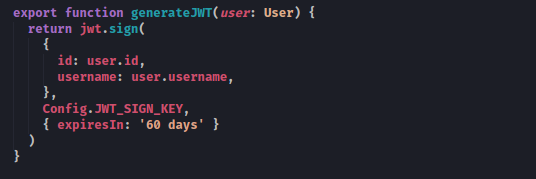
\includegraphics[width=\textwidth]{generate_jwt.png}
  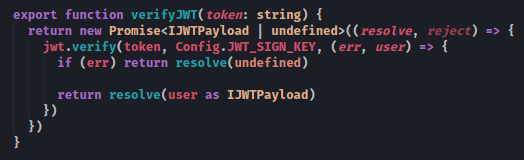
\includegraphics[width=\textwidth]{verify_jwt.png}
  \caption{Generiranje i verificiranje tokena}
\end{figure}

\myparagraph{Baza}
Za pohranu korisnika koristi se \foreign{SQLite} baza podataka.
\paraBreak
Ova baza je odabrana primarno zbog svoje jednostavnosti, naime za razliku od ostalih baza koje funkcioniraju na
klijent-poslužitelj modelu, ova baza je kompletno ugrađena u jednu datoteku. \cite{SQLite} \\
Zbog jednostavnosti i malog broja entiteta poslužitelja ova baza je idealno rješenje.

\begin{figure}[h]
  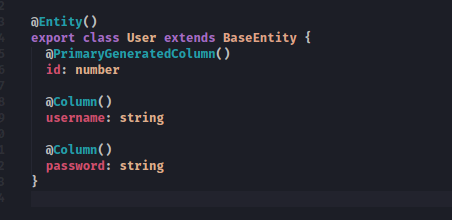
\includegraphics[width=\textwidth]{user_entity.png}
  \caption{User entitet koji predstavlja tablicu u bazi}
\end{figure}

\begin{figure}[h]
  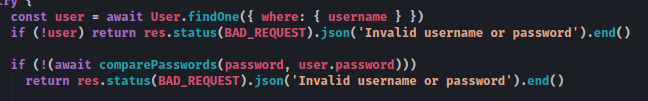
\includegraphics[width=\textwidth]{get_user.png}
  \caption{Dohvaćanje korisnika iz baze i provjera lozinke}
\end{figure}

\begin{figure}[h]
  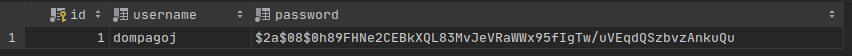
\includegraphics[height=1.5cm, width=\textwidth]{user_table.png}
  \caption{Tablica korisnika u bazi}
\end{figure}

\clearpage
\subsubsection{Komunikacija sa transkoderom} \label{sec:http}
Primarni način kojim poslužitelj komunicira sa transkoderom je TCP (\foreign{Transmission Control Protocol}) protokol. \\
Jedan glavnih i naj zastupljenijih protokola weba povrh kojeg je HTTP protokol implementiran. \cite{webProtocols}
\paraBreak
Nudi pouzdanu vezu u kojoj se za razliku od UDP protokola, primljeni paketi provjeravaju za redoslijed, odnosno TCP
garantira da su svi primljeni paketi stigli istim redoslijedom kojim su i poslani, što je u slučaju video prijenosa jako bitno. \\
\paraBreak
TCP je baziran na konekcijama odnosno veza između klijenta i poslužitelja je uspostavljena prije nego se paketi mogu slati, ovo je
glavni razlog zašto je odabran umjesto UDP protokola koji nudi bolje performanse. Naime jedan od ciljeva je imati
podršku za više kamera odnosno traskodera, što je s TCP-om trivijalno za implementirati, dok bi se s UDP-om moralo
implementirati vlastiti sustav identifikacije svakog paketa.
\paraBreak
Klasa \keyword{StreamingClients} predstavlja listu svih spojenih transkodera odnosno kamera, sadrži metode:
\begin{itemize} \label{sec:sreaming_clients}
  \item \keyword[o]{addClient} - dodaje novog klijenta
  \item \keyword[o]{removeClient} - briše klijenta
  \item \keyword[o]{getClient} - dohvaća klijenta
  \item \keyword[o]{getClients} - vrača listu svih klijenata
\end{itemize}
Privatno polje \keyword[p]{clients} je mapa svih klijenata kojoj je ključ jedinstveni identifikator klijenta, dok
je vrijednost klasa \keyword{CameraStream}. Ona sadrži dva polja \keyword[p]{header} i \keyword[p]{socket}.
\paraBreak
Kada se nova kamera spoji putem tcp-a u ovu mapu pod nasumično generiranim ključem koji predstavlja
jedinstveni identifikator spojene kamere sprema se nova instanca klase \keyword{CameraStream} pozivom metode
\keyword[o]{addClient}, u polje \keyword[p]{socket} sprema se pokazivač na samu TCP konekciju, dok se polje
\keyword[p]{header} puni isključivo prvim paketom kojeg je ta kamera poslala, zato što transkoder prije nego
počne slati pakete samog videa, prvo šalje zaglavlje. \ref{sec:output_format_ctx}
\paraBreak
Zaglavlje se pohranjuje na ovaj način jer ga je potrebno poslati za svaki HTTP zahtjev prije samih paketa videa kako
bi klijentov video player znao prikazati video.
\clearpage
\begin{figure}
  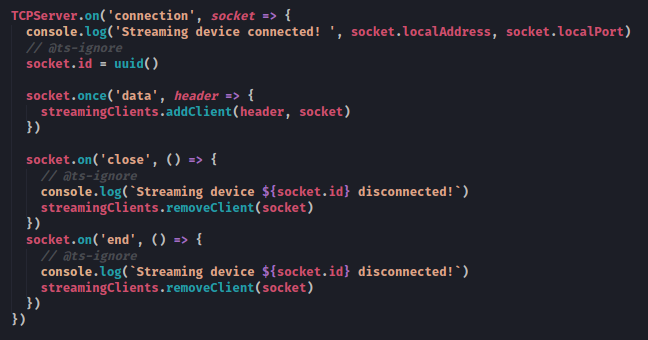
\includegraphics[width=\textwidth]{tcp_connections.png}
  \caption{Obrađivanje TCP konekcija}
\end{figure}

\begin{figure}
  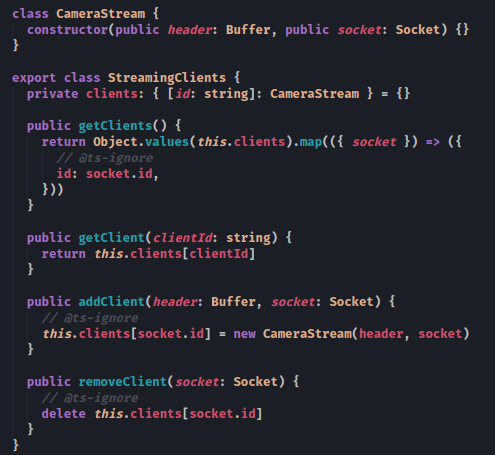
\includegraphics[width=\textwidth, height=10cm]{streaming_clients.png}
  \caption{Klase StreamingClients i CameraStream}
\end{figure}
\clearpage
\subsubsection{Prijenos klijentima}
Primarni način kojim poslužitelj komunicira s klijentima je HTTP (\foreign{Hypertext Transfer Protocol}) protokol.
\paraBreak
Ovaj protokol je temelj podatkovne komunikacije weba, baziran na zahtjev-odgovor principu gdje klijent primjerice
web preglednik šalje zahtjev nekom poslužitelju koji zauzvrat vrača odgovor u obliku HTML teksta, datoteke i ostalo.
\paraBreak
Format klijentskog zahtjeva se sastoji od rute koja predstavlja željeni resurs, primjerice '/korisnici', zaglavlja
zahtjeva, metoda, te opcionalno tijelo zahtjeva.
Metoda predstavlja tip akcije koji klijent želi odraditi, najbitnije od kojih su:
\begin{itemize}
  \item GET - dohvaćanje resursa, ne smije na nikakav način modificirati sam resurs
  \item POST - kreiranja novog resursa
  \item PUT - ažuriranje postojećeg resursa
  \item DELETE - brisanje resursa
\end{itemize}

\myparagraph{Rute} \label{sec:routes}
Na ovom poslužitelju postoje 4 glavne rute
\begin{itemize}
  \item [GET] /streams - vrača listu svih aktivnih kamera te njihove identifikatore, očekuje JWT token u zaglavlju
  \item [GET] /streams/:id/watch - vrača video podatke konkretne kamere ovisno o \\ 
    parametru \foreign{id} koji predstavlja identifikator kamere
  \item [POST] /auth/login - ruta za prijavu korisnika
  \item [GET] /auth/me - vrača podatke o korisniku dobivene iz tokena poslanog u zaglavlju
\end{itemize}
\noindent
Ruta \foreign{/watch} ne očekuje JWT token u zaglavlju jer zahtjev na ovu rutu u slučaju web preglednika vrši
\foreign{HTML5} video player nad kojim klijent nema kontrolu, zbog toga se token šalje kroz samu rutu u obliku
/watch?token='token'
\paraBreak
Sam proces slanja videa ove rute se odvija na sljedeći način:
\begin{enumerate}
  \item Verifikacije tokena iz rute
  \item Pronalaženje kamere po identifikatoru poslanom u ruti, u slučaju da kamera ne postoji poslužitelj odmah odgovara
    sa HHTP odgovorom 400 (bad request)
  \item Postavljanje zaglavlja odgovora \foreign{Content-Type} na video/webm
  \item Zapisivanje zaglavlja videa iz dohvaćene kamere u odgovor
  \item Prosljeđivanje ostatka podataka iz kamere u odgovor
\end{enumerate}

\begin{figure}[h]
  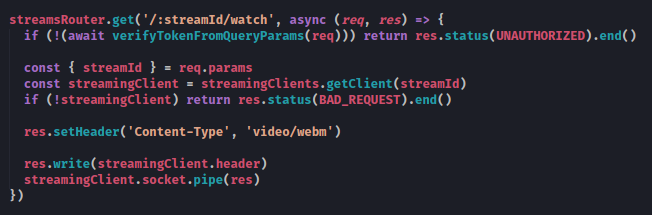
\includegraphics[width=\textwidth]{watch_endpoint.png}
  \caption{HTTP ruta za slanje videa}
\end{figure}